\section{Related works}

\begin{frame}{Information Retrieval}
    
    \begin{figure} [H]
        \begin{center}
            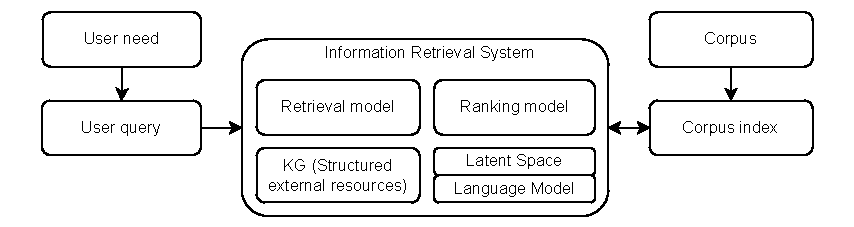
\includegraphics[scale=0.8]{images/ir-system-comps.pdf} 
            \caption{Information Retrieval System overview} 
        \end{center}
    \end{figure}

    \begin{center}
        Traditional approaches leverage statistics about the text corpus. Recent methods implement deep learning models and combines multiple approaches.
    \end{center}
    
\end{frame}

\begin{frame}{BM25}
    
    BM25 (and its many variants) is:
    \begin{itemize}
        \item based on the Term Frequencies and Inverse Document Frequencies (TF-IDF)
        \item still widely used in practice
        \item computes many statistics offline
    \end{itemize}

    \begin{center}
        Traceparts search system is largely based on a BM25 implementation.
    \end{center}
    
\end{frame}

\begin{frame}{Knowledge Graph and ontology}

    Knowledge Graph (Hogan et. al. 2021):
    \emph{a knowledge graph is a graph of data intended to accumulate and convey knowledge of the real world, whose nodes represent entities of interest and whose edges represent relations between these entities.}
    % \emph{a knowledge graph is a graph of data intended to accumulate and convey knowledge of the real world, whose nodes represent entities of interest and whose edges represent relations between these entities. The graph of data (aka. data graph) conforms to a graph-based data model, which may be a directed edge-labelled graph, a property graph, etc. By knowledge, we refer to something that is known.}

    Ontology (Hogan et. al. 2021):
    \emph{In the context of computing, an ontology is then a concrete, formal representation of what terms mean within the scope in which they are used (e.g., a given domain).}

    \begin{center}
        In our work, we consider an ontology a particular component of a Knowledge Graph
    \end{center}
    
\end{frame}